\chapter{Сводное дерево успешных, закрытых и проверяемых ветвей}

После ретроспективного и negative-space аудитов состояние программы удобнее
фиксировать не линейным списком, а деревом зависимостей. Зелёные узлы
обозначают воспроизводимое математическое ядро, жёлтые --- условные
кандидаты, красные --- закрытые реализации, синие --- оставшиеся decisive
gates, фиолетовые --- архитектурные коррекции.

\begin{landscape}
\begin{figure}[p]
 \centering
 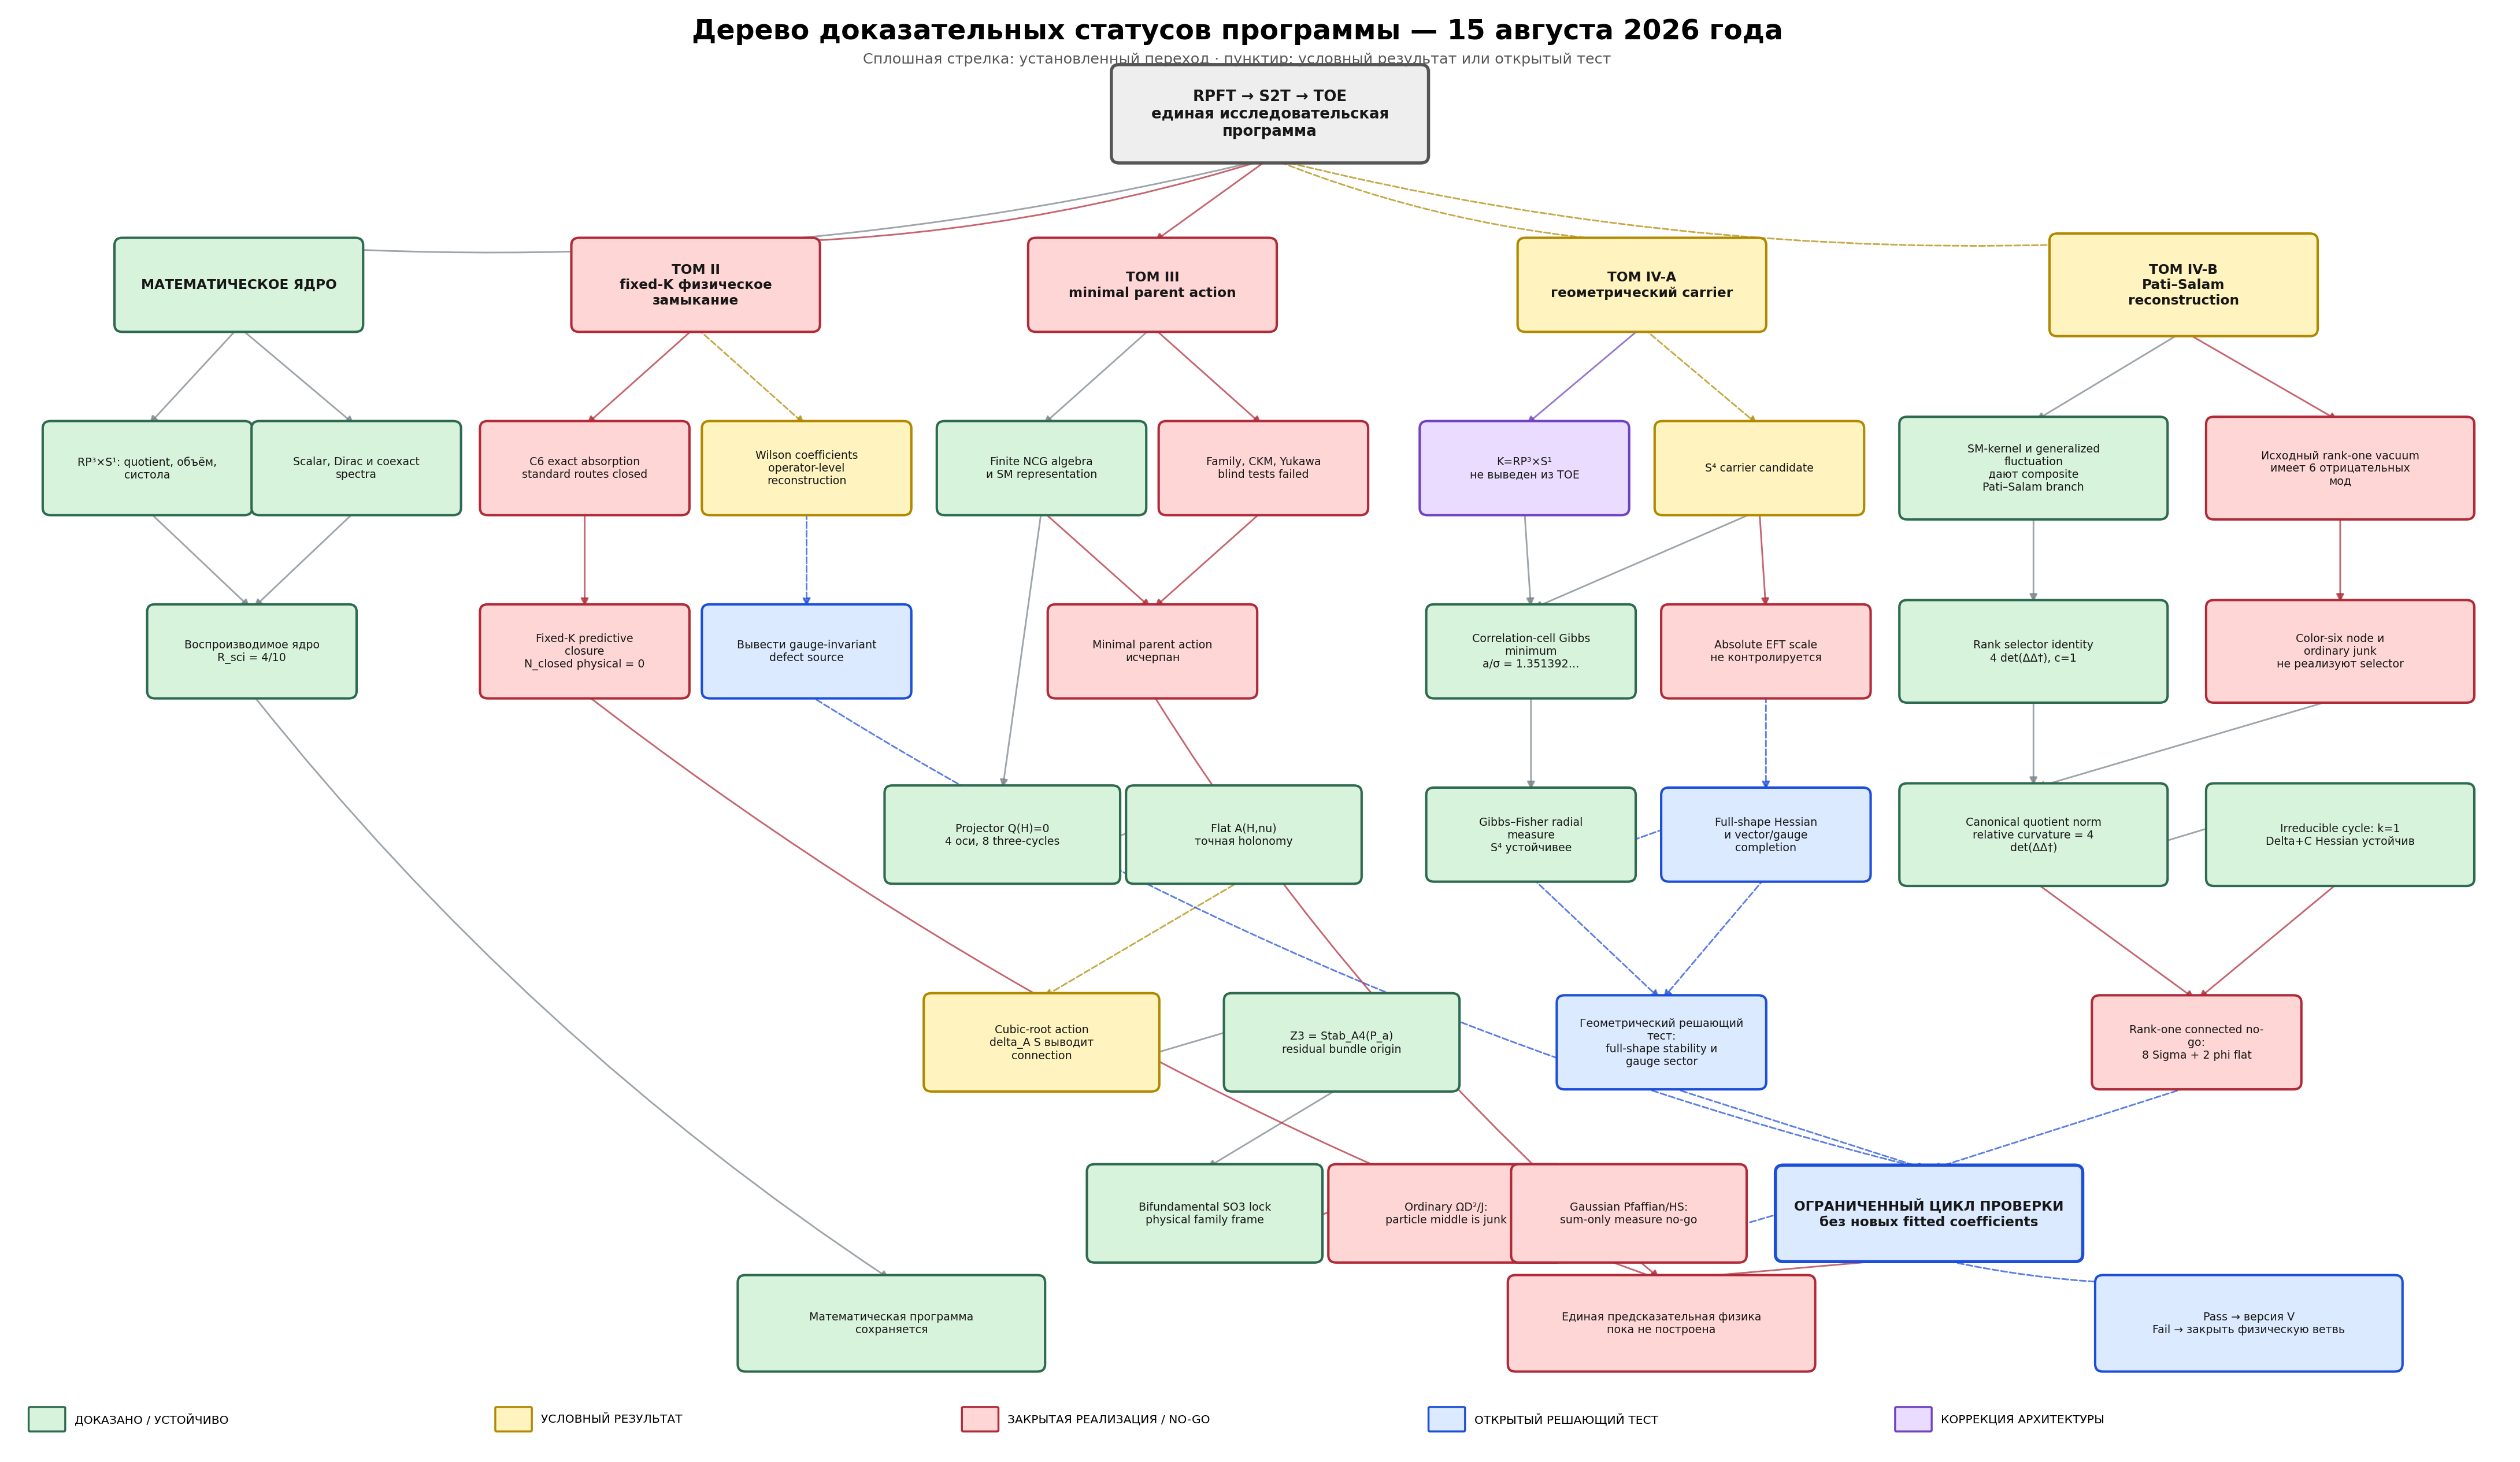
\includegraphics[width=0.97\linewidth,keepaspectratio]{fig_project_success_tree_v4_current_2026-08-15.png}
 \caption{Дерево доказательных статусов программы по состоянию на
 15 августа 2026 года. Pati--Salam reconstruction выделена в отдельную
 ветвь; цвет кодирует доказательный статус, а не численную вероятность.}
 \label{fig:project-success-tree-v4}
\end{figure}
\end{landscape}

Главный смысл рисунка~\ref{fig:project-success-tree-v4} состоит в разделении
двух итогов. Математическая программа не обнулена: geometry, spectra,
\(Q_{\rm cycle}\), \(\mathbb Z_2\)-данные и Gibbs--Fisher radial measure
сохраняются. Физическое замыкание остаётся нулевым:
\begin{equation}
 R_{\rm sci}=4/10,
 \qquad
 N_{\rm closed\ physical}=0.
\end{equation}

После reverse-audit красный цвет означает закрытую конкретную реализацию или
доказанный no-go, а не отсутствие научного результата. Поэтому нейтринный
узел разделён на сохранённую topology/operator часть и замороженную
количественную ветвь; EW/QCD переведён в conditional status из-за
непроверенного quadratic \(T_{3R}^2\) parent class.

Новый Gauss-law audit разделил два вопроса. Relative normalization допускает
согласованное completion: полный family-traced functional равен
\(3V_{\rm gap}\), если tree и periodic sectors также несут triplet
multiplicity. Но один diagonal \(U(1)\) constraint имеет nullity семь, а два
irrep-block constraints --- nullity шесть. Они не выбирают единственный
momentum vector \(1^3 3^5\). Для прежнего product integral нужен новый
rank-eight covariant projector.

Альтернативная конструкция использует один sixteen-mode Gaussian carrier с
axis-coherent source нормы $48$ одновременно даёт inverse term и log
determinant. Fixed-charge rotors и rank-eight projector для этой ветви не
нужны. Открытым остаётся происхождение imaginary defect source из
gauge-invariant parent action.

Последний ограниченный цикл теперь состоит из четырёх открытых узлов:
\begin{enumerate}
 \item gauge-invariant origin coherent imaginary defect source;
 \item global nonlocal spectral-metric origin;
 \item full-shape Fisher/Kubo Hessian;
 \item massive-vector completion и RG evolution от spectral boundary.
\end{enumerate}

Минимальный relative topology prior закрыт как trivial-or-free menu.
Symmetric \(U(2)\) interaction-sign gate закрыт точной factorization
\begin{equation}
 Z_{\rm prod}-Z_{U(2)}=(E_3-O_3)O_1>0.
\end{equation}
Первым открытым gate теперь является происхождение coherent defect source;
затем следуют global spectral metric, full-shape Hessian и
vector-completion/RG.

Литературная sign-коррекция уточняет global spectral branch. Negative Hessian
free energy по external source является стандартным signed response, а
positive susceptibility равна его минусу. Поэтому mapping-cone coefficient
\(-(1-c)/45\) сохраняется как exact zero-source two-point response даже при
наличии higher determinant powers. Открытым остаётся response-to-action gate:
parent theory должна потребовать именно эту stiffness observable, а не full
determinant при unit source.

Новый архитектурный audit уточняет последний RG-узел. Родственная успешной
части проекта spectral Pati--Salam ветвь является наиболее экономным
кандидатом на UV transmission layer, но не готовым решением. При фиксации
уже полученного масштаба \(m_R=1.0317\times10^{13}\,\mathrm{GeV}\) четыре
канонических scalar scenarios оставляют \(2.63\%\)--\(4.90\%\) spread.
Exact one-loop unification возвращается только при свободном выборе
\(m_R\). Поэтому следующий blue gate --- вывести Pati--Salam vacuum и
\(m_R\) из finite Dirac/scalar action, заморозить scenario и лишь затем
повторить blind RG test.

Vacuum gate уже сужает этот маршрут. Опубликованный spectral Pati--Salam
potential оставляет required Goldstone mass-degenerate с unwanted scalar.
Существующий Coleman--Weinberg singlet в minimal direct sum развязан, а
universal portal не меняет разность этих масс. Кроме того, условный
нейтринный \(M_R^{(0)}=2.4637\,\mathrm{GeV}\) отстоит от Pati--Salam
scales на \(10.78\)--\(13.31\) порядков. Поэтому новый blue gate --- не
singlet tuning, а перебор representation-sensitive diagonal finite blocks,
одновременно способных расщепить scalar sectors и вывести transmutation
scale.

Первый group-theory diagnostic непуст. Identity singlet имеет нулевую
различимость, тогда как \(C_2[SU(2)_R]\) и \(C_2[SU(4)]\) дают разность eigenvalues
\(-2\) между unwanted \((0,\mathbf6)\) и required
\((1,\mathbf{10})\) modes. Первым кандидатом выбран единый four-color
diagonal block \(\mathbf1\oplus\mathbf{15}\). Но Casimir difference не
является вычисленной mass matrix конкретного VEV; открыт полный
spectral-potential/Hessian gate.

Первичный representation audit исправляет этот optimistic status. Поле
\(\Sigma\) текущего spectral menu имеет
\((2_R,2_L,1+15_4)\), поэтому его high-scale VEV разрушает weak
\(SU(2)_L\) и порождает large Dirac masses. Breaking через \(\dot H\)
оставляет девять required и шесть unwanted massless modes, а остальные
Hessian directions отрицательны. Для general branch нужен иной dynamic
sector; composite \((1,1,15)\) и diagonal singlet должны проверяться после
построения явного project Dirac block с полным potential.

Повторный literature audit разделил scenario ledger. Weak-singlet
\((1,1,15)\) действительно присутствует в constrained composite branch,
но не как independent field general fundamental branch. Поэтому vacuum
no-go остаётся строгим для fundamental potential, а composite branch
переходит в conditional status: нужно вывести first-order reduction из
явного project Dirac block и включить composite/nonrenormalizable terms.
Diagonal real singlet также остаётся открытым extension, тогда как закрыт
только pure universal mass-shift ansatz.

Следующий foundational gate частично закрыт конструктивно. На
\(V_R\oplus V_L\oplus V_R^c\oplus V_L^c\) complex dimension 32 построен
explicit KO6 block с channels \(Y,M_R,M_L\). Он проходит self-adjointness,
odd grading и reality и автоматически даёт fundamental representations
\((2,2,1+15)\), \((3,1,10)+(1,1,6)\) и left counterpart. Composite
\(\phi,\Delta,\Sigma_4\) ansatz является нелинейным restricted image:
27 complex coordinates в complexification или 39 real degrees при
Hermitian adjoint condition, внутри 200-real-dimensional active
\(Y+M_R\) space. Открыт exact
first-order double-commutator kernel.

Exact kernel теперь вычислен. На 272-real-dimensional KO6 Dirac space full
Pati--Salam algebra оставляет dimension 8:
\(Y=A\otimes I_4\), \(M_R=M_L=0\). Embedded SM subalgebra оставляет
dimension 32: independent lepton/quark bidoublet blocks и один
\(\Delta\sim(2_R,4_4)\)-подобный symmetric Majorana seed, при \(M_L=0\).
Результат проходит exhaustive algebra-basis test и four-convention scan.
Открыт generalized inner-fluctuation gate для вывода nonlinear
\(\Sigma_4\) и \(\Delta\Delta\).

Generalized inner-fluctuation gate теперь закрыт конструктивно. После
ограничения на normalized self-adjoint semigroup
\(\operatorname{Pert}(\mathcal A_{PS})\) unitary-orbit identity выполняется
с ошибкой порядка \(10^{-15}\), тогда как удаление \(A_{(2)}\) даёт
order-one mismatch. На физическом seed linear ranks равны (8) для
bidoublet \(\phi\) и (16) для \(\Delta(2_R,4_4)\). Каждый full Yukawa
point имеет weak--color reshuffle rank два с tilde-invariant weak subspace,
а каждый right-Majorana point имеет crossed reshuffle rank один:
\(H_{\dot aI\dot bJ}=k^{\nu_R*}\Delta_{\dot aJ}\Delta_{\dot bI}\).
Следовательно, composite Pati--Salam branch действительно выведен из exact
project Dirac block; следующим открытым gate становится вычисление полного
composite spectral potential и его vacuum Hessian.

Этот vacuum gate теперь также вычислен. При сохранении weak \(SU(2)_L\)
необходимо \(\phi=0\), после чего composite \(\Sigma_4\) исчезает из finite
operator и остаётся flat. Для \(\Delta\) physical half-traces равны
\(\rho^2\) и \(\tau^2\), поэтому normalized potential имеет вид
\(V=-\rho^2+\tau^2\). Желаемый rank-one orbit имеет Hessian signature
\((1_+,9_0,6_-)\), тогда как lower rank-two orbit имеет
\((4_+,12_0,0_-)\), но неправильный unbroken subgroup. Любая singlet
поправка только через \(\rho\) сохраняет отрицательный rank-growth mode.
Тем самым minimal fundamental и minimal composite spectral Pati--Salam
vacua закрыты. Открыта только расширенная geometry, способная вывести
rank-sensitive determinant invariant или independent connected adjoint.

Project archaeology нашла точный непараметрический rescue candidate.
Direct и crossed quadratic \(\Delta\)-paths удовлетворяют identity
\(\|H^{\rm dir}-H^{\rm cr}\|^2=4\det(\Delta\Delta^\dagger)\). Полученный
coefficient \(\kappa=4\) меняет rank-one Hessian signature с
\((1_+,9_0,6_-)\) на \((7_+,9_0,0_-)\) и удаляет lower rank-two stationary
branch. Независимо combined \(SU(2)_R+SU(4)\) Casimir gap между
\((3,10)\) и \((1,6)\) также равен четырём. Поэтому potential-level repair
найден; новый blue gate --- вывести direct/crossed relative sign из одного
KO6-compatible doubled-path Krajewski block или graded superconnection без
свободного coefficient.

Wedge-channel compatibility gate закрывает representation-level сомнение.
Raw direct-minus-crossed matrix симметрична и проходит self-adjointness,
odd grading и KO6 reality в существующем \(M_R\)-slot. В rank-one vacuum
она обращается в нуль, её Jacobian имеет rank шесть, а девятимерная gauge
orbit и radial direction лежат в kernel. Поэтому selector действует ровно
на шесть bad modes, не меняет Goldstone count и tree-level fermion masses.
Единственный оставшийся blue gate --- явный doubled-path parent graph,
который выводит relative sign и coefficient четыре.

Этот parent-graph gate дал минимальный equivariant carrier.
Трёхузловая exterior-square chain
\(\mathbb C\to(2,4)\to(1,6)\) имеет KO6 completion и проходит coarse
order-one label test. Её ordinary half-traces равны
\begin{equation}
 \frac12\Tr D_F^2=\frac72\rho,
 \qquad
 \frac12\Tr D_F^4=\frac{19}{8}\rho^2+\frac72
 \det(\Delta\Delta^\dagger),
\end{equation}
а rank-one Hessian имеет signature \((7_+,9_0,0_-)\). Механизм устойчив
при \(0<c^2<8\), поэтому это не одна подогнанная normalization point.
Однако associative-module audit закрывает literal Krajewski interpretation:
\(\Lambda^2\) является representation группы, но не complex-linear unital
representation \(M_4(\mathbb C)\), а любой nontrivial color module этой
matrix algebra имеет dimension, кратную четырём. Поэтому color-six не может
быть новым fermion node. Сохранённый blue route --- получить тот же
\((1_R,6_4)\) selector как represented universal two-form или curvature
component внутри существующего 32-dimensional Hilbert module после quotient
по degree-two junk, затем пересчитать mixed
\((\phi,\Sigma_4,\Delta)\) Hessian.

Первый differential-calculus audit закрывает три прямых продолжения.
Ordinary represented two-forms являются grading-even, тогда как wedge
Majorana block grading-odd; junk quotient parity не меняет. Physical
Standard-Model seed даёт только crossed reshuffle rank one. Общий
16-real-dimensional SM Majorana seed, наоборот, раздувает quadratic
\(A_{(2)}\)-image до всех 72 real dimensions symmetric \(8\times8\)
Majorana channel. Поэтому direct и wedge paths появляются только вместе со
всеми competitors. Оставшийся blue gate --- вычислить even gauge-singlet
sector degree-two quotient и проверить, содержит ли его curvature norm
\(\det(\Delta\Delta^\dagger)\). При norm-only результате следует перейти к
vectorlike extension из допустимых fundamental \(4\) и \(\bar4\) modules.

Project archaeology нашла эту extension в уже существующих механизмах.
Минимальная chain
\begin{equation}
 \bar4^+\longrightarrow2_R^-\longrightarrow4^+
\end{equation}
использует только допустимые fundamental/opposite modules. При edges
\(A_\Delta=\Delta\) и
\(B_\Delta=c\Delta^T\varepsilon_2\) endpoint curvature равна color-six
matrix \(c\Delta^T\varepsilon_2\Delta\), а её relative norm даёт
\begin{equation}
 \|F_{02}\|^2=4c^2\det(\Delta\Delta^\dagger).
\end{equation}
При canonical metric \(c=1\) восстанавливается exact coefficient четыре;
rank-one Hessian устойчив уже при \(c^2>1/2\). Full ordinary trace при этом
остаётся rank-blind, поэтому recovery принадлежит projected superconnection
curvature class. Новый blue gate --- вывести endpoint projector и equality
metrics из одного parent action, затем проверить physical/auxiliary status
vectorlike modules, mixed Hessian и gauge running.

Junk/mapping-cone audit разделяет две части этого blue gate. Map
\(\Delta\mapsto\Delta^T\varepsilon_2\) является Frobenius-isometry, а
endpoint reflection/reality фиксирует \(c=1\) без continuous weight.
Standard node differential calculus не даёт требуемый projector: для
\(\mathbb C^3\) path represented two-form rank равен пяти, junk rank ---
двум, причём \(E_{02},E_{20}\) лежат в junk. Зато path Laplacian имеет
единственную reflection-odd coordinate \(h=(-1,0,1)\), и normalized
mapping-cone derivative
\begin{equation}
 \delta_h(F)=\frac12[h,F]
\end{equation}
канонически оставляет только endpoint curvature. Поэтому
\begin{equation}
 \|\delta_h(\mathcal D_\Delta^2)\|^2
 =4\det(\Delta\Delta^\dagger).
\end{equation}
Fixed-point quotient gate закрывает этот выбор на уровне relative geometry:
\begin{equation}
 \inf_{C\in\mathcal B_h}\|F-C\|^2
 =\|F-E_h(F)\|^2
 =\left\|\frac12[h,F]\right\|^2
 =4\det(\Delta\Delta^\dagger)
\end{equation}
на even curvature space. При общем sector weight
\(\lambda_{\rm rel}\) transverse Hessian положителен для
\(\lambda_{\rm rel}>1/2\).

BV/multiplicity audit закрывает standard gauge-fixing auxiliary как источник
этого веса и показывает, что relative chain отсутствует как hidden submodule
стандартного Pati--Salam fermionic space. Поэтому decisive gate является
архитектурным fork. Physical vectorlike branch anomaly-safe, но после shift
\((\Delta b_R,\Delta b_L,\Delta b_4)=(-2/3,0,-4/3)\) не проходит
one-percent fixed-scale RG test. Classical mapping-cone branch не добавляет
propagating states и при one-copy trace даёт \(\lambda_{\rm rel}=1\), но
one-copy multiplicity должна быть выведена из parent geometry. После выбора
одной ветви требуется полный mixed Hessian и RG/threshold ledger.

Irreducible-cycle gate выбирает classical branch без нового coefficient.
Для \(k\) одинаковых copies commutant connected operator system равен
\(M_k(\mathbb C)\), поэтому irreducibility выполняется только при
\begin{equation}
 k=1,
 \qquad
 \lambda_{\rm rel}=1.
\end{equation}
Полный Hessian до устранения fixed-point auxiliary curvature имеет
\(16+36=52\) real variables и inertia
\begin{equation}
 (43_+,9_0,0_-).
\end{equation}
Его Schur complement точно возвращает effective spectrum
\(8\sqrt2\ (1),2\sqrt2\ (6),0\ (9)\). Тем самым identical-copy fork и
auxiliary instability закрыты. Новый blue gate --- встроить relative cycle
в полную KO6 real structure и вычислить оставшиеся mixed
\(\phi/\Sigma_4\) directions; physical vectorlike branch сохраняется только
как отдельная расширенная model при отказе от minimal irreducibility.

KO6/full-Hessian gate отделяет algebraic compatibility от physical vacuum.
Relative chain допускает exact \(20\)-dimensional KO6 completion и сохраняет
coefficient четыре после physical half-trace. Но ordinary direct-sum reading
добавляет двадцать finite fermionic states, поэтому non-propagating branch
должна оставаться relative bosonic/KK cycle.

Главный результат отрицателен уже на уровне общего quadratic form:
\begin{equation}
 H_Y(Y)=-4\|Y\|^2+8\|M_R^\dagger Y\|^2\le0,
 \qquad
 \|M_R\|_{\rm op}^2=\frac12.
\end{equation}
Project \(\phi\)-tangent имеет восемь negative modes, а Hermitian traceless
\(\Sigma_4\) даёт пятнадцать flat directions. Полный исследованный ledger
равен
\begin{equation}
 (43_+,24_0,8_-).
\end{equation}
Таким образом, determinant selector ремонтирует \(\Delta\), но current full
composite vacuum закрыт. Следующий threshold gate уточняет purple correction
node. Connected scalar channel \(\zeta\|Y\|^2\) устраняет все восемь
\(\phi\)-instabilities только при \(\zeta>2\); при этом все пятнадцать
\(\Sigma_4\)-directions остаются flat. Поэтому следующий минимальный target
--- twisted scalar--vector parent, который одним fixed spectral mechanism
даёт как scalar shift выше порога, так и direct representation-sensitive
\(\Sigma_4\)-potential. Если этот target не проходит, остаётся genuine
two-scale spectral action; менять coefficient rank selector повторно не
допускается.

Project-wide archaeology дополнительно закрывает два apparent shortcuts.
Для common spectral family
\(V_\alpha=-(\alpha/2)\Tr D_F^2+(1/2)\Tr D_F^4\) все восемь negative
\(\phi\)-eigenvalues только умножаются на \(\alpha\), а пятнадцать
\(\Sigma_4\)-directions остаются flat. Twisted grand-symmetry model из
литературы является Pati--Salam-like algebra с \(M_3(\mathbb C)\),
Majorana singlet и spacetime vector, а не full \(SU(4)\) adjoint mechanism.
Поэтому purple node теперь требует mixed relative curvature, которая одним
fixed trace weight создаёт \(\zeta_Y>2\) и full-rank
\(\Sigma_4\)-Hessian. Если такой invariant не возникает, one-copy relative
rescue закрывается и требуется новая fundamental diagonal finite geometry.

Следующий coefficient audit обнаруживает дополнительное ограничение.
Канонический graded tensor product фиксирует mixed quartic coefficient
точно \(c=4\), то есть \(\zeta=c/2=2\). Это устраняет negative directions,
но оставляет четыре \(\phi\)-zero modes и не даёт strict vacuum. Повторение
двух identical copies подняло бы коэффициент до \(8\), однако породило бы
copy commutant \(M_2(\mathbb C)\) и нарушило one-copy irreducibility.
Поэтому purple node теперь допускает только derived higher spectral moment
с полной radial restationarization либо non-identical auxiliary factor со
scalar joint commutant. В противном случае tensor-product rescue закрыт.

Финальные два gates закрывают обе возможности внутри current geometry.
Для любого radial polynomial stationarity тождественно даёт
\(\zeta=2\alpha\), поэтому higher moments оставляют четыре
\(\phi\)-zero modes. Для genuinely connected contractions единственный
rank-one color projector имеет общий \(\mathfrak{su}(3)\)-stabilizer:
полный \(\Sigma_4\)-span имеет rank \(7\) и восемь flat directions, а
полный connected \(\phi\)-span имеет rank \(6\) и две flat directions.
Таким образом, Pati--Salam node становится red: current finite geometry
закрыта. Rank-\(\ge3\) diagonal carrier или несколько noncommuting
projectors относятся уже к Version V.

Rotation audit старых проблем меняет рабочий порядок, но не статусы дерева.
Первым приоритетом становится family--defect boundary superconnection:
условие continuous \(SO(3)\) сокращает двенадцать full-\(M_3\) affine
candidates до восьми three-cycles, одновременно сохраняя exact-one
Majorana core mechanism. Existing Wilson axes не совпадают с discrete
three-cycle axes, поэтому требуется новый parent selection gate, а не
переименование уже найденного решения.

Первый gate этого приоритета теперь даёт conditional positive result.
Кубический \(S_4\)-инвариант и zero-character condition образуют
неотрицательный functional с четырьмя минимумами для каждого знака unit
vortex winding. Два winding sectors дают ровно восемь three-cycles при
угле \(2\pi/3\), а каждый generator имеет rank два и оставляет один
Majorana core mode. Открытым остаётся supertrace-origin: три слагаемых
functional должны возникнуть из одной graded boundary curvature, а не быть
добавлены как независимые potentials.

Projector-supercurvature factorization объединяет radial и axis conditions.
Equation \(Q(H)=H^2-H/\sqrt3-I_4/4=0\) имеет ровно четыре rank-one
projector solutions на affine menu. Вместе с двумя winding orientations
они реконструируют восемь three-cycles и проходят все 192
twisted-covariance tests. Новый decisive gap состоит в получении cycle как
actual holonomy той же graded connection, а не как post-processing rule.

Flat-holonomy gate закрывает этот algebraic gap на constrained saddle.
Operator \(\Omega(h)=*(u\wedge h)\) строится из affine singlet,
projector-selected axis и orientation tensor. Connection
\(\mathcal A=-\nu(2\pi/3L)\Omega(h)ds\) имеет holonomy ровно выбранный
three-cycle, коммутирует с \(H\) и сохраняет exact-one kernel. Поэтому
следующий decisive gap состоял в выводе constitutive relation
\(\mathcal A=\mathcal A(H,\nu)\) из одного parent action.

Cubic-root action gate проходит этот criterion в фиксированном condensed
unit-winding sector. Frame
\begin{equation}
 W=\exp\!\left[\frac{\varphi}{3}\Omega(H)\right]
\end{equation}
имеет \(\mathbb Z_3\)-transition, а variation единого positive functional
\begin{equation}
 S_{\rm root}=\int ds\left[
 L^{-1}\Tr Q(H)^2+L\Tr\!\left((D_sW)^TD_sW\right)
 \right]
\end{equation}
даёт
\begin{equation}
 \mathcal A_s=-\partial_sW\,W^T
 =-\frac{\partial_s\varphi}{3}\Omega(H).
\end{equation}
Тем самым connection--projector dependence больше не является ansatz;
holonomy зависит только от winding, а connection Hessian положителен.

Новый blue gate лежит глубже: вывести nonzero pairing condensate,
cubic-root bundle и его embedding в finite graded superconnection из одного
parent action. Пока этот carrier принят как boundary-sector input,
family--defect branch остаётся conditional и не меняет
\(N_{\rm closed\ physical}=0\).

Tetrahedral residual-bundle gate теперь закрывает discrete degree этого
carrier. Четыре axes образуют regular tetrahedron и канонически задают
spin-three tensor с proper stabilizer \(A_4\). После выбора \(P_a\)
остаётся
\begin{equation}
 \operatorname{Stab}_{A_4}(P_a)
 =\{1,C_{a,+},C_{a,-}\}
 \simeq\mathbb Z_3.
\end{equation}
Все четыре stabilizers и оба orientations проверены машинно; binary lifts
имеют order six. Поэтому factor \(1/3\) больше не является отдельным
дискретным input.

Открытый узел одновременно стал точнее. Global \(A_4\) сохраняет physical
различимость axes, но не создаёт gauge bundle. Gauged residual \(A_4\)
создаёт order-three flux, однако axes становятся gauge-related без
boundary framing. Поэтому следующий blue gate --- вывести gauged или
boundary-framed tetrahedral carrier вместе с nonzero ordinary charge-two
\(B-L\) defect condensate из одного finite graded parent action.

Gauge--family locking gate закрывает axis-framing часть. Real
bifundamental \(X\) с vacuum \(X\in SO(3)\) ломает
\(SO(3)_{\rm gauge}\times SO(3)_{\rm family}^{\rm global}\) до exact
diagonal global group. Его Hessian равен \((6_+,3_0,0_-)\), а три gauge
masses положительны и равны в canonical normalization. Поэтому residual
\(\mathbb Z_3\) flux теперь имеет physical family frame без перехода к
новой family \(SU(3)\) gauge algebra.

Оставшийся blue gate стал одномернее. Общая symmetry разрешает effective
pairing mass обоих знаков и не заставляет \(B-L\) field конденсироваться.
Coefficient-free candidate
\begin{equation}
 V_\mu=\left(|\Phi|^2-\frac13\Tr X^TX\right)^2
\end{equation}
автоматически даёт nonzero condensate в locked vacuum, но ratio
\(1:-2/3:1/9\) должен быть получен из одного central curvature или finite
graded supertrace. Именно этот parent-trace calculation теперь является
следующим decisive family--defect gate.

Quiver moment-map gate проходит этот calculation в explicit
frozen--gauged--frozen chain. \(A_4\)-Schur lemma фиксирует pairing arrow
как \(Y=\Phi I_3\), а middle curvature
\begin{equation}
 \mu_G=XX^T-|\Phi|^2I_3
\end{equation}
даёт exact identity
\begin{equation}
 \frac13\Tr\mu_G^2
 =\left(|\Phi|^2-\frac13\Tr XX^T\right)^2
 +\frac13\Tr\left(XX^T-\frac13\Tr(XX^T)I_3\right)^2.
\end{equation}
Тем самым ratio \(1:-2/3:1/9\) выведен, а не выбран. Zero-gradient
Hessian равен \((7_+,4_0,0_-)\). После включения unit defect momentum
joint radial minimum остаётся condensed и лежит ниже normal branch на
\(0.0013020084\).

KO6 embedding gate закрывает representation-level часть. Explicit
18-dimensional real-even completion проходит self-adjointness, grading,
reality, order-zero и first-order conditions. Более того, first-order
condition сам оставляет одномерный commutant и потому выводит
pairing arrow
\begin{equation}
 Y=\Phi I_3,
\end{equation}
а не принимает его как внешний Schur ansatz.

Одновременно ordinary spectral-action route закрывается отрицательно. На
radial slice \(X=\rho I_3\), \(\Phi=r\) получено
\begin{align}
 \Tr D_p^4&=6(\rho^2+r^2)^2,\\
 \frac13\Tr\mu_G^2&=(\rho^2-r^2)^2.
\end{align}
Следовательно, ordinary trace имеет положительный mixed quartic, тогда как
moment-map curvature требует отрицательный. Quadratic spectral term знак
не меняет, а \(\Str D_p^4=0\). Поэтому finite representation существует,
но требуемый condensate не является следствием стандартного
one-trace polynomial этого \(D_F\).

Новый blue gate теперь уже не algebraic embedding. Требуется вывести
incoming-minus-outgoing middle curvature как canonical auxiliary
\(D\)-sector или relative/mapping-cone action и одновременно доказать, что
его trace normalization совпадает с kinetic normalization полей \(X\) и
\(\Phi\). После этого нужно повторить full nonradial и BdG audit.

Relative/auxiliary audit показывает, что эта формулировка была ещё слишком
широкой. Canonical mapping-cone norm от \((d+d^\dagger)^2\) сохраняет
endpoint composition и равен
\begin{equation}
 2|\Phi|^2\Tr XX^T,
\end{equation}
поэтому не содержит pure quartics и закрывается. Strict
\(SO(3)\)-adjoint D-term также закрывается: требуемая
\(\mu_G=XX^T-|\Phi|^2I_3\) симметрична, тогда как
\(\mathfrak{so}(3)\) состоит из skew matrices, и adjoint projection равна
нулю.

Условно положительным остаётся более точный self-adjoint auxiliary route.
На каноническом module \(\operatorname{Sym}_3(\mathbb R)\) выполнено
\begin{equation}
 \tau_3(\mu_G^2)
 =\sup_{K=K^T}\{2\tau_3(K\mu_G)-\tau_3(K^2)\},
\end{equation}
причём stationary field равен \(K=\mu_G\), а та же \(\tau_3\) нормирует
kinetic terms \(X\) и \(\Phi\). Новый blue gate --- вывести этот
six-dimensional self-adjoint module и его единственную trace metric из
represented degree-two junk quotient или uniquely fixed BV complex. Только
после этого auxiliary construction станет parent-geometry result.

Повторный literature audit существенно сужает и исправляет этот узел.
Matrix
\begin{equation}
 \mu_J=XX^T-|\Phi|^2I_3
\end{equation}
остаётся точным middle Hodge commutator, но на declared real \(SO(3)\)
field space не является strict Hamiltonian moment map: её contraction с
каждым skew generator \(\mathfrak{so}(3)\) равна нулю. Поэтому unitary
quiver D-term literature не даёт прямого parent proof для real branch.

Canonical mapping-cone norm также закрывается: он равен только
\begin{equation}
 2|\Phi|^2\Tr XX^T
\end{equation}
и не содержит pure quartics. Self-adjoint Legendre identity формально
reproduces \(\tau_3(\mu_J^2)\), но её auxiliary Hessian имеет шесть
eigenvalues \(-2/3\). Real positive auxiliary minimum даёт quartic
противоположного знака.

Explicit junk quotient закрывает первый route. На generic фоне represented
two-form rank равен двадцати, junk rank --- девяти, quotient rank ---
одиннадцати. На particle half весь middle \(M_3\) лежит в junk; full KO6
quotient сохраняет только одну central conjugate direction и не содержит
traceless symmetric module.

Финальная проверка фермионной меры закрывает второй маршрут. Самостоятельная
конечная KO6-билинейная форма симметрична, поэтому её грассманова
антисимметричная часть равна нулю. После четырёхмерного пополнения
\begin{equation}
 \log|\operatorname{Pf}\mathcal D_p|
 =3\log p^2+6\log(p^2+\rho^2+r^2),
\end{equation}
а все even moments зависят только от \(\rho^2+r^2\). Поэтому Gaussian
measure не различает points \((1,0)\) и
\((2^{-1/2},2^{-1/2})\), тогда как moment-map square равен на них единице
и нулю. Loop quartic имеет ratio \(1:2:1\), а не \(1:-2:1\).

Таким образом, family--defect parent route внутри Version IV закрыт.
Reopening требует four-fermion channel, modified calculus, Cartan torsion
либо нового finite carrier и относится к Version V.

Исходный machine-readable graph сохранён в
\path{project_success_tree_v4_results.json}; генератор рисунка ---
\path{generate_project_success_tree_v4.py}.
